% Document type and package imports.
\documentclass[ebook, 8pt, oneside, openany]{memoir}
\usepackage[utf8]{inputenc}
\usepackage[T1]{fontenc}
\usepackage[french]{babel}
\usepackage{charter}
\usepackage[top = 2cm, bottom = 2cm, left = 1cm, right = 1cm]{geometry}
\DisemulatePackage{setspace}
\usepackage{setspace}
\usepackage{url}
\usepackage{color}
\usepackage{graphicx}
\usepackage{makeidx}
\usepackage{wrapfig}
\usepackage{hyperref}
\usepackage{makeidx}
\usepackage{fancyhdr}
\usepackage[svgnames]{xcolor}
\usepackage{titlesec}
\usepackage{xhfill}

% Preanblue.
\onehalfspacing \definecolor{gray}{rgb}{0.4, 0.4, 0.4} \colorlet{rulecolor}{Gainsboro!40!Lavender}
\hypersetup {colorlinks=true, linkcolor=black, urlcolor=black, pdftitle={Cahier des charges de Godot Mega Assets}} \lhead{\textit{GODOT MEGA ASSETS}} \fancyfoot[CE,CO]{} \rfoot{Page \thepage}
\pagestyle{fancy} \rhead{\textbf{2021 - 2022}} \renewcommand{\headrulewidth}{2pt} \renewcommand{\footrulewidth}{1pt} \lfoot{\textit{Edité par Prince Obrymec}}
\titleformat{\chapter}[display]{\filcenter}{\mbox{}\xrfill[0.4ex]{3pt}[rulecolor]\textsc{\large\enspace\chaptername \thechapter}\enspace\xrfill[0.4ex]{3pt}[rulecolor]\mbox{}}{0.3ex} {{\color{rulecolor}\titlerule[1pt]}\vskip3ex\huge\bfseries}[\medskip{\color{rulecolor}\titlerule[1pt]}]
\renewcommand*{\chaptitlefont}{\normalfont\LARGE\bfseries} \definecolor{darkblue}{RGB}{65, 90, 110}
\definecolor{darkred}{RGB}{110, 65, 65} \definecolor{darkgreen}{RGB}{10, 90, 65}
\definecolor{darkorange}{RGB}{110, 90, 65}

% The start of the book.
\begin{document}
	% Generates table of contents and table of figures.
	\tableofcontents \pagebreak \listoffigures
	
	% Spécifications.
	\chapter{\textcolor{darkblue}{Ingénierie du cahier des charges}}
	% Area analytics.
	\section{\textcolor{darkred}{Analyse du domaine}}
	% Area actors.
	\subsection{\textcolor{darkorange}{Les acteurs du domaine}}
	Les créateurs de jeux vidéo ne sont pas seulement des informaticiens: c'est aussi le résultat du travail
	de \textit{graphistes}, de \textit{chefs de projets}, et de métiers plus \textit{spécialisés}, comme
	\textit{ergonome}, ou \textit{game designer}.
	% Game designer.
	\subsubsection{\textcolor{darkgreen}{Le Game Designer}}
	C'est le garant de la cohérence du jeu. Il s'assure que le projet reste cohérent, réfléchit aux
	interactions possibles et à ce qui améliorera l'expérience de jeu. Il réfléchit à ce que l'expérience
	apportera au joueur, et à la manière dont le jeu peut être amélioré, enrichi, ou simplifié.
	% Developper.
	\subsubsection{\textcolor{darkgreen}{Le Programmeur}}
	Si le game designer est celui qui dit \textbf{on pourrait...}, le programmeur est souvent celui qui dit 
	\textbf{on ne pourra pas}. Responsable des choix techniques, il doit savoir quelles sont les
	possibilités offertes par un langage ou un outil, et trouver les astuces qui rendront le
	\textbf{théoriquement impossible} possible.
	% Graphic designer.
	\subsubsection{\textcolor{darkgreen}{Le Graphiste}}
	Avec le responsable du son, le graphiste détermine l'ambiance générale du jeu. Une tâche qui ne fait pas 
	seulement appel à des choix esthétiques: le graphisme est intimement lié aux choix conceptuels.
	% Ergonoma.
	\subsubsection{\textcolor{darkgreen}{L'Ergonome}}
	\textbf{Si le joueur joue mal, c'est de notre faute}: la formule est ironique, mais elle est en partie 
	juste. L'ergonome est responsable de la maniabilité et de la bonne compréhension du joueur. C'est lui 
	qui s'assure que l'objectif d'une mission, par exemple, est suffisamment clair, et qui invente les
	formes de suggestion utilisées pour indiquer au joueur ce qu'il peut ou ne peut pas faire.
	% Project manager.
	\subsubsection{\textcolor{darkgreen}{Le Chef de projet}}
	Chef d'orchestre de l'équipe, le chef de projet est aussi celui qui garde à l'esprit les containtes 
	économiques: quel type de marketing ferait connaître le jeu ? Quel budget nécessiterait telle ou telle
	modification ? A quel marché sera destiné le jeu ?
	% Graphic designer.
	\subsubsection{\textcolor{darkgreen}{L'Infographite 2D/3D}}
	Métier créatif, \textbf{l'infographie} a le vent en poupe dans le milieu vidéoludique. Très similaire au
	métier de \textbf{graphiste}, \textbf{l’infographiste} réalise des \textbf{décors}, des
	\textbf{personnages} ou des \textbf{interfaces} de jeux vidéo. Contrairement au \textbf{graphiste}, son
	métier peut s’exercer principalement dans l’industrie du jeu vidéo ou de l’animation. Il est, en
	général, celui qui va appliquer les consignes du \textbf{game designer}. Il va dessiner ses croquis, les
	présenter à sa direction ou au \textbf{chef de projet} puis les mettre en forme grâce à différents
	outils numériques de \textbf{PAO} qu’il doit parfaitement maîtriser.
	% Animator 2D/3D.
	\subsubsection{\textcolor{darkgreen}{Animateur 2D/3D}}
	C'est également un artiste qui s’occupe de l’animation d’un jeu vidéo et est responsable d’animer des
	personnages, un décor des objets ou d’une interface du jeu en développement. C’est en quelque sorte le
	professionnel du mouvement de l’industrie des jeux vidéo. Parmi ses nombreuses tâches, il a la charge de
	rendre un jeu réaliste si besoin est. Les expressions faciales de personnages, il les connaît: c’est lui
	qui les fait. La roulade de Link, il connaît c’est lui qui l’a faite. Il s’occupe de la fluidité du jeu
	et qui le rend «vivant». L’animateur maîtrise sur le bout des doigts tous les logiciels d’animation 3D
	et 2D et peut créer des images de synthèse en volume.
	% Business Developer.
	\subsubsection{\textcolor{darkgreen}{Business Developer}}
	Ce métier diffère quelque peu de ceux traités précédemment, mais son rôle est pourtant primordial. Ne
	touchant pas à la partie créative de la conception d’un jeu vidéo, le \emph{business developer} peut 
	travailler en agence de jeux vidéo. Il s’occupe de la relation avec les clients. Il est notamment
	responsable d’identifier et de trouver de nouveaux partenaires. Il peut établir la stratégie à suivre
	d’une agence et rechercher de nouvelles opportunités de business. Il doit également aller sur les
	différents salons et événements de jeu vidéo pour présenter sa marque et la faire \textbf{rayonner}.
	% QA developpement.
	\subsubsection{\textcolor{darkgreen}{Testeur développement/QA}}
	Job de rêve pour certains gamers, le testeur de jeux vidéo est surtout un professionnel indispensable
	dans la chaîne de production d’un jeu vidéo. Le testeur développement est responsable de la vérification 
	de la jouabilité d’un jeu vidéo. Il s’assure donc de la qualité du \textbf{gameplay} et doit détecter le 
	moindre bug d’un jeu. Il a la charge d'examiner chaque détail d’un jeu vidéo. La première image que vous 
	vous faites de ce métier commence à changer ? C’est normal, ce métier demande beaucoup de patience, un 
	testeur doit essayer toutes les configurations d’un jeu vidéo, faire, refaire les mêmes choses. Imaginez 
	pour un jeu vidéo en monde ouvert. Il doit ainsi déceler les problèmes et les reporter afin que les
	programmeurs, designers, game designers les rectifient. C’est en quelque sorte un critique du jeu vidéo 
	qui doit être bon communicant.
	% Associate producer.
	\subsubsection{\textcolor{darkgreen}{Associate producer}}
	Ce professionnel travaille au sein de l’équipe de production d’un jeu vidéo. Il est sous la direction 
	d’un producteur et ses missions sont principalement de \textbf{manager} les équipes afin qu'elles 
	suivent les priorités établies sur les \textbf{plannings}. Ainsi, il s'occupe du \textbf{suivi} de la 
	production tout en veillant au respect de la \textbf{qualité} exigée, du \textbf{budget} ainsi que du 
	\textbf{temps} qui est imposé aux équipes. Il doit ainsi faire un bilan régulier à son supérieur pour 
	l’informer de l’état de la production. Il peut également assurer la communication entre les différentes 
	équipes d’un projet et participer au recrutement.
	
	% Game Engine description.
	\subsection{\textcolor{darkorange}{Description du système existant et fonctionnement}}
	Notre système vise l'industrie du jeu vidéo. Cepandant, notons qui existe déjà des solutions apportées
	dans ce domaine à travers l'utilisation de progiciels appelés \textbf{Game Engine} ou \emph{moteur de
	jeu} en français. Un \textit{moteur de jeu} est un ensemble de composants logiciels qui effectuent des 
	calculs de géométrie et de physique utilisés dans les jeux vidéo. L'ensemble forme un simulateur en 
	temps réel souple qui reproduit les caractéristiques des mondes imaginaires dans lesquels se déroulent 
	les jeux. Le but visé par un moteur de jeu est de permettre à une équipe de développement de se
	concentrer sur le contenu et le déroulement du jeu plutôt que la résolution de problèmes informatiques.
	Le moteur 3D crée des images par des calculs de projection, tandis que le moteur 2D construit l'image du 
	jeu par empilement d'images matricielles. Le moteur effectue le mixage des bruits et de la musique tout 
	au long du jeu. Les possibilités de scriptage des moteurs de jeu permettent de simuler le comportement
	des personnages non-jouables avec peu ou pas de programmation et le moteur physique sert à appliquer des 
	règles de physique telles que l'inertie ou la pesanteur dans le but d'obtenir des mouvements plus
	réalistes. Dans les jeux vidéo modernes, il existe des ensembles principaux parfois gérés par des 
	moteurs distincts, chacun concernant une fonction spécifique du développement: le système (entrée/
	sortie, interface utilisateur, mémoire, etc.), le graphisme, le son, le réseau (\textit{pour les jeux
	multijoueurs}), la physique et l'intelligence artificielle.\\
	Chaque moteur de jeu est unique. Toutefois, certaines fonctionnalités se retrouvent:
	% Library resources.
	\subsubsection{\textcolor{darkgreen}{Les ressources de la bibliothèque}}
	Les systèmes de moteur de jeu 3D sont mis en œuvre en assemblant de nombreuses bibliothèques de
	ressources. Le développeur du moteur sélectionne un moteur de jeu en fonction de ses bibliothèques de
	ressources de programmation disponibles. Une bibliothèque commune pour un moteur de jeu 3D simple se
	compose de graphiques 3D, de physique, de détection de collision, d'entrée/sortie, d'audio, d'IA, de
	graphiques 3D et d'une bibliothèque réseau. Les moteurs de jeu modernes peuvent inclure des
	bibliothèques plus puissantes, notamment des lois physiques, la détection de collision et des effets
	spéciaux. De plus, les ressources du moteur de jeu contiennent des exemples de projets, des guides
	d'utilisation et des didacticiels; ces ressources disponibles sont extrêmement utiles pour un
	développeur de jeux.		
	% Input output manager.
	\subsubsection{\textcolor{darkgreen}{Le gestionnaire d'entrées/sorties}}
	Cette partie s'occupe de la lecture des périphériques externes:
	\begin{itemize}
		\item[• Joystick:] Lecture de l'état des boutons et du ou des sticks;
		\item[• Souris:] Lecture de l'état des boutons, du mouvement relatif, de la position;
		\item[• Clavier].
	\end{itemize}
	Elle est aussi chargée de la lecture des données du jeu, et de l'écriture des sauvegardes:
	\begin{itemize}
		\item[• Lecture/écriture depuis un disque dur];
		\item[• Lecture depuis un DVD, un CD ou un mini disk];
		\item[• Lecture/écriture depuis une carte mémoire].
	\end{itemize}
	C'est elle qui se chargera de compresser/décompresser les données du jeu (notamment pour accélérer les
	chargements). Elle sera aussi chargée de leur éventuel chiffrement/déchiffrement.
	% Maths.
	\subsubsection{\textcolor{darkgreen}{Les mathématiques}}
	On y trouvera toutes sortes de fonctions mathématiques nécessaires à l'élaboration d'un jeu. Pour un jeu 
	3D, on y trouvera plus particulièrement:
	\begin{itemize}
		\item[• \textbf{\textcolor{blue}{Les matrices}}:] En général, des matrices 3x4 ou 4x4 pour le
		stockage de l'orientation des objets (sur les trois axes), de leur échelle (sur les trois axes) et
		parfois aussi de leur position. La signification réelle des lignes et colonnes est directement liée
		au moteur et n'a pas toujours de base mathématique réelle. Certains stockeront une échelle uniforme
		sur la dernière colonne ou ligne, d'autres la translation, d'autres encore utiliseront des matrices
		de transformations plus complexes pour éviter les problèmes d'échelle dans le cas des matrices
		hiérarchisées.
		\item[• \textbf{\textcolor{blue}{Les quaternions}}:] Ils servent au stockage des orientations. Ils
		sont beaucoup plus compacts que les matrices et supportent beaucoup mieux les interpolations. On les
		retrouve typiquement dans les animations, pour stocker l'orientation de chaque clef d'interpolation.
		\item[• \textbf{\textcolor{blue}{Les vecteurs}}:] À deux, trois ou quatre dimensions. On parle de
		composantes x, y, z et w. La composante w n'est en général pas utilisée, et n'existe qu'à des fins
		d'optimisation sur les processeurs 128 bits. On peut citer comme exemple de calcul très souvent
		effectué dans un moteur de jeu : la multiplication de matrices, l'inversion de matrices, le produit
		scalaire ou vectoriel.
	\end{itemize}
	% Physic.
	\subsubsection{\textcolor{darkgreen}{La physique}}
	Le module de physique calculera le mouvement des objets, la manière dont ils interagissent les uns avec 
	les autres, la manière dont ils glissent sur le sol ou sur les murs, la manière dont ils rebondissent, 
	etc. C'est lui aussi qui calculera la déformation des objets mous, des cheveux, poils, vêtements et 
	autres rideaux. On peut distinguer trois grandes catégories de simulation:
	\begin{description}
		\item[• \textcolor{blue}{La physique du point}:] C'est la plus simple. Un objet est formalisé par un
		seul point en mouvement avec une vitesse, une accélération, une friction, de la gravité, etc. En
		général, ce genre de physique se contente de déplacer les objets sans agir sur leur orientation;
		\item[• \textcolor{blue}{La physique du solide}:] Chaque entité est formalisée par une ou plusieurs
		primitives géométriques (boîte, sphère, gélule, cylindre) ou même par une enveloppe (maillage
		quelconque) éventuellement convexe. La physique du solide est beaucoup plus réaliste (et donc
		complexe) que la physique du point puisqu'elle gère aussi l'évolution de l'orientation. Certains
		éditeurs se sont spécialisés dans la fabrication de modules de physique du solide pouvant être
		directement intégrés dans les moteurs existants. On citera par exemple \textbf{Havok},
		\textbf{Novodex} et dans le domaine du libre \textbf{ODE} ou \textbf{Bullet};
		\item[• \textcolor{blue}{La physique des particules}:] Elle s'apparente à la physique du point. Un
		volume est constitué d'un ensemble de particules (on parle aussi d'atomes) liées entre eux par des
		contraintes (le plus souvent des ressorts). Ce type de physique autorise la déformation et la
		rupture de volume. Elle est donc particulièrement bien adaptée à la simulation des tissus.
	\end{description}
	% Collisions detection.
	\subsubsection{\textcolor{darkgreen}{La détection des collisions}}
	La gestion des collisions est une couche logicielle qui permet de détecter lorsque deux objets se
	rencontrent et ainsi de pouvoir définir une action résultante. Un objet est alors une représentation
	géométrique d'éléments du jeu (personnages, obstacle, projectiles...). Un module de collision est
	typiquement constitué d'un ensemble de fonctions mathématiques pour le calcul des intersections par
	paires de primitives géométriques: sphère contre sphère, sphère contre boîte, boîte contre triangle...
	Chacune de ces fonctions calculera selon les capacités du module le point d'intersection, la normale au
	point de contact, ainsi que la distance de pénétration des deux objets. On distingue deux grandes
	catégories de collisions:
	\begin{description}
		\item[• La détection sur modèle d'objets \textcolor{blue}{statiques}:] La plus simple, considère que
		deux objets sont en collision si au moment du traitement de la détection les deux objets se
		touchent. Comme le traitement est échantillonné régulièrement dans le temps, des objets en mouvement
		rapide ont très bien pu entrer en contact avec d'autres objets entre deux temps d'échantillonnage.
		\item[• La détection sur modèle d'objets \textcolor{blue}{dynamiques}:] S'attache aussi au mouvement
		des objets. On traite la transition d'un instant échantillonné au suivant. Les calculs sont plus
		coûteux, mais ont l'avantage d'empêcher un volume en mouvement d'en traverser un autre sans que cela
		soit détecté. L'instant de la collision de deux objets peut être calculé plus précisément qu'avec la
		technique dite statique.
	\end{description}
	Selon le type de jeu l'une ou l'autre des approches est utilisée. Les moteurs de jeu en 3D actuels
	utilisent typiquement un mélange de ces deux méthodes. Pour optimiser les calculs de collision sur les
	formes complexes, les moteurs de jeu peuvent utiliser la notion de volume englobant et plus généralement
	de hiérarchie de volumes englobants. Le calcul rapide mais approximatif permet alors d'éliminer des
	états de non collision, dans le cas contraire un calcul exact est réalisé sur l'objet. La hiérarchie de
	volumes englobants rajoute seulement des étapes supplémentaires en subdivisant un objet en sous
	ensembles englobés dans une forme simple. Pour réduire le nombre de calcul de paire d'objets les moteurs
	recourent généralement à structurer l'espace en sous ensembles d'objets proches.
	% Render engine.
	\subsubsection{\textcolor{darkgreen}{Les graphismes}}
	Dans les jeux en 3 dimensions, les scènes et les objets du jeu (monstres, véhicules, projectiles) sont
	enregistrés sous la forme des coordonnées en 3 dimensions de polygones — souvent des triangles. Chaque
	suite de polygones forme les contours des différents objets du monde du jeu. Le moteur 3D effectue des
	calculs de \textbf{synthèse d'image} en vue d'obtenir une projection en 2 dimensions du monde du jeu,
	projection qui sera envoyée à l'écran. Dans le procédé dit du rendu polygonal (ou rasterisation), le
	moteur 3D effectue le calcul de la \textbf{projection} à partir d'un point de vue donné, en commençant
	par les polygones les plus éloignés de ce point de vue. La texture (couleur, motifs...) des surfaces est
	une \textbf{image matricielle} déformée en fonction de la distance et l'orientation du polygone par
	rapport au point de vue avant d'être appliquée sur la projection. Dans le procédé dit voxel (contraction
	de volume et pixel), les objets du jeu sont enregistrés sous forme d'une suite de cubes (les voxels) et 
	le calcul de la projection utilise le procédé du rendu polygonal. Dans le procédé dit du lancer de rayon
	(ou ray tracing), le moteur 3D effectue le calcul de la couleur de chaque pixel de la projection (qui
	est une \textbf{image matricielle}) en calculant en sens inverse le chemin parcouru par la lumière pour
	chaque pixel de l'image, conformément aux règles de \textbf{l'optique géométrique} telles de que
	transparence, la réflexion ou la réfraction. Ce procédé donne des images très réalistes, mais il demande
	une grande puissance de calcul et, en 2011, il est encore peu utilisé pour les jeux vidéo. Les calculs
	de projection peuvent être effectués par le processeur graphique (abr. \textbf{GPU}) pendant que le
	processeur central est utilisé pour d'autres calculs tels que ceux du moteur son ou du scriptage.
	% Sound manager.
	\subsubsection{\textcolor{darkgreen}{La gestion du son}}
	Le moteur sonore combine un logiciel de \textbf{lecteur audio} avec un logiciel de \textbf{mixage} et un
	générateur d'\textbf{effets sonores} (écho, compression, spatialisation). Les trois composants sont
	interconnectés. Le moteur son effectue en continu des calculs de \textbf{synthèse sonore} et de
	\textbf{traitement numérique du signal}, sur la base d'\textbf{échantillons} (sample) numérisés, de 
	partitions musicales (souvent au format \textbf{MIDI}) et de \textbf{tables d'ondes}. Certains moteurs 
	son simulent la \textbf{réverbération}, le \textbf{déphasage}, et le changement de timbre d'un son émis
	par une source éloignée, et produisent ainsi des \textbf{illusions auditives}.
	% Scripting.
	\subsubsection{\textcolor{darkgreen}{Le scriptage}}
	Les \textbf{langages de script} sont souvent utilisés dans les jeux vidéo pour programmer le
	comportement des ennemis ou des machines et ainsi simuler leur \textbf{intelligence}. Le recours à un
	langage de script permet à un designer ou un scénariste, qui a peu ou pas de connaissance en
	programmation, de «configurer» le comportement des ennemis et ainsi modifier le \textbf{gameplay} sans 
	faire appel à un programmeur. Historiquement, le besoin d'un système de script s'est fait sentir pour
	les jeux d'aventure nécessitant beaucoup d'interactions. Il en a découlé \textbf{Script Creation Utility
	for Maniac Mansion} (SCUMM). Créé initialement, et comme son nom l'indique pour le jeu \textbf{Maniac
	Mansion} (1987), et réutilisé pour chaque nouveau jeu avec un minimum de modifications, il a resservi
	dix ans plus tard pour le jeu \textit{The Curse of Monkey Island} (1997). Les autres genres de jeu sont
	aussi devenus à leur tour complexes, leurs moteurs de jeu ont alors souvent incorporé un système de
	script. Pour le développement de \textit{Jedi Knight}: \textit{Dark Forces II} (1997), le moteur de jeu
	a été adapté pour supporter un langage de script. \textbf{Robert Huebner}, qui a participé à cette
	évolution, explique qu'il existait avant cela un langage binaire INF qu'il était dur d'assimiler — un
	livret complet était destiné à cet usage. Le langage de script implémenté, COG, est compilé à la volée
	lors du lancement d'une partie puis exécuté sur une \textbf{machine virtuelle} (un \textbf{automate} à
	pile) pour assurer la robustesse du jeu. Il n'y a eu aucune conséquence négative rapportée que ce soit
	sur le développement ou sur le jeu lui-même, mais plutôt un accroissement de la créativité des
	concepteurs. Certaines entreprises ont développé leurs propres langages de script, comme il est écrit
	plus haut. C'est aussi le cas d'id Software avec le langage \textbf{QuakeC} ou d'\textbf{Epic Games}
	avec le langage \textbf{UnrealScript}. Mais l'intégration d'un langage de script est devenue très
	accessible, certaines bibliothèques logicielles étant développées indépendamment spécialement dans ce
	but. C'est le cas de la bibliothèque et du langage \textbf{Lua} qui a été utilisé dans un grand nombre
	de jeux de genres très divers.
	% Modularity	
	\subsubsection{\textcolor{darkgreen}{La modularité}}
	Le moteur de jeu doit être implémenté via plusieurs modules uniques. Chaque composant du gestionnaire
	est indépendant un peu comme une seule unité fonctionnelle. Les développeurs de moteurs doivent investir
	du temps dans la mise en œuvre d'une architecture de jeu modulaire pour réduire la complexité du système
	et offrir de la robustesse. Le processus de test et la maintenance deviennent plus faciles pour le
	programmeur en cas de besoin.
	% Usability.
	\subsubsection{\textcolor{darkgreen}{L'usabilité}}
	Les développeurs de moteurs sont les principaux acteurs; par conséquent, la convivialité d'un moteur de
	jeu est un critère important à évaluer. L'utilisabilité inclut la facilité d'apprentissage, l'efficacité
	d'utilisation, la mémorabilité, la fréquence et la gravité des erreurs, et la satisfaction subjective.
	La facilité d'apprentissage et l'efficacité d'utilisation sont les principaux aspects de la
	convivialité.
	% Efficiency.
	\subsubsection{\textcolor{darkgreen}{Efficacité}}
	L'efficacité du moteur de jeu fait référence à l'utilisation réussie de toutes les entrées et des
	ressources disponibles pour produire une sortie de jeu donnée. Il comprend l'allocation de mémoire,
	l'utilisation du processeur, le processus de rendu et d'autres fonctionnalités. Nous pouvons produire un
	moteur efficace mais pas un jeu efficace. En effet, le flux de travail du jeu est conçu par le créateur
	du jeu, ce qui a un impact sur l'efficacité du jeu. Les gestionnaires de ressources jouent un rôle
	important pour ce critère. Il charge les données et les fichiers du jeu du disque dans la mémoire pour
	être utilisés pour le rendu et la création de scénarios de jeu. Les concepteurs de jeux devraient
	considérer les concepts de réutilisabilité et de modularité pour améliorer l'efficacité du moteur. Des
	ressources uniques peuvent être utilisées pour créer de nombreuses instances.
	% Rendering effects and picture quality.
	\subsubsection{\textcolor{darkgreen}{Effets de rendu et qualité d'image}}
	Le processus de rendu produit des graphiques animés en 3D à l'aide de techniques spécifiques telles que
	la rastérisation, le rendu basé sur l'image (IBR), le lancer de rayons ou toute autre technique. Ces
	techniques sont précieuses pour les moteurs de jeux 3D. Contrairement aux graphiques 2D, la mise en
	œuvre d'un rendu graphique 3D nécessite des compétences avancées en programmation et en modélisation 3D.
	Les graphiques 3D ont d'innombrables algorithmes de rendu d'extrêmement rapide à extrêmement lent. Le
	rendu matériel et logiciel a un impact sur l'accélération des graphismes 3D. La plupart des moteurs
	disponibles rendent une scène en utilisant les paramètres par défaut. Ces fonctionnalités peuvent être
	utiles pour un aperçu rapide, mais pas pour le travail de production. Avec les moteurs modernes, vous
	pouvez obtenir une sortie très nette, claire et de haute qualité; cela se fait au prix d'un temps de
	rendu accru même si le rendu final sera bien meilleur.

	% Game engine existing models.
	\subsection{\textcolor{darkorange}{Le model existant du domaine}}
	Un moteur est une partie essentielle d'un jeu; il influence la structure et l'organisation des
	graphiques du jeu, des fichiers de configuration et de toutes les autres entrées telles que les entrées
	utilisateur, les cartes et les sons. La figure ci-dessous montre un diagramme de composants d'un moteur
	de jeu dans un contexte de développement de jeu.
	\begin{figure}[h]
		\begin{center}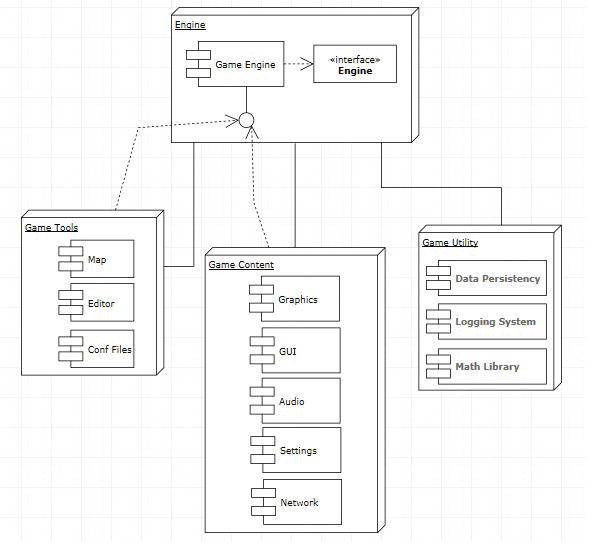
\includegraphics[height = 225pt]{game_engine_components_diagram.png}\end{center}
		\caption{Diagramme des composants d'un moteur de jeu}
		\label{Diagramme des composants d'un moteur de jeu}
	\end{figure}
	\\Les outils de jeu, l'utilitaire de jeu et le contenu du jeu sont également des composants essentiels
	d'un jeu. Les outils de jeu font référence à tous les outils utilisés pour développer un jeu, tels que 
	l'éditeur de personnage, l'éditeur de capacité, les fichiers de configuration et la carte du jeu. Le
	contenu du jeu fait référence à toutes les fonctionnalités associées dans n'importe quel jeu. Les
	fichiers graphiques et audio sont le type de données le plus important. Les composants réseau permettent
	à plusieurs utilisateurs de se connecter les uns aux autres et d'accéder aux données du jeu. Les
	composants utilitaires définissent tous les types de données, formats de message et fichiers requis, en
	fonction des caractéristiques du jeu. Le composant outil de jeu joue un rôle de pont entre le contenu du
	jeu et les composants du moteur de jeu. Actuellement, aucune architecture standard spécifique n'a été
	développée dans la théorie. La figure ci-dessous montre une architecture détaillée d'un moteur de jeu.
	Nous ne considérons que certaines caractéristiques qui sont probablement importantes.
	\begin{figure}[h]
		\begin{center}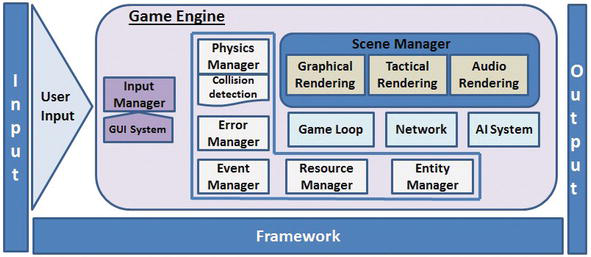
\includegraphics[height = 150pt]{detailed_game_engine_architecture.png}\end{center}
		\caption{Architecture détaillée d'un moteur de jeu}
		\label{Architecture détaillée d'un moteur de jeu}
	\end{figure}
	\\Les composants du gestionnaire sont essentiels à tous les jeux. Une mangeoire physique est importante
	pour les jeux dépendant de réactions physiques. Par exemple, la course automobile a besoin de lois
	physiques, mais ce n'est pas si important pour un jeu d'association de cartes. Cependant, le
	gestionnaire d'entrée et le système d'interface graphique sont importants, même pour un jeu simple, pour
	traiter l'entrée de l'utilisateur. Le gestionnaire de scène est tenu d'organiser et de contrôler le
	contenu de la scène et de surveiller la logique du jeu. La boucle de jeu est utilisée pour contrôler une
	boucle infinie qui fait tourner le jeu encore et encore. Le composant réseau est responsable de la
	gestion des connexions des utilisateurs et de l'accès aux données de jeu (Multijoueur). Le système AI
	est un module spécial conçu et écrit par des ingénieurs logiciels possédant des connaissances
	spécialisées. Des composants de gestionnaire supplémentaires, qui dépendent du programmeur et des
	approches de codage comme les états du jeu, le moteur de règles et la reconnaissance vocale, peuvent
	être nécessaires à des moments spécifiques.

	% Game Engine requirements.
	\subsection{\textcolor{darkorange}{Les ressources nécessaires à un moteur de jeu}}
	Utilisé un moteur de jeu est comme joué à un jeu vidéo à cause de la possibilité de tester le jeu au
	cours de son développement. Cette fonctionnalité est présente dans tous les moteurs de jeux. Ainsi la
	nécessité de détenir les bons outils pour les utilisés. Qui parle d'outils, parlera forcement d'un
	ordinateur, car c'est ce qu'il faut pour utilisé un moteur de jeux. Cepandant, les spécifications
	requises de votre machine dépendent totalement du type de jeu que vous souhaitez créer et du moteur avec
	lequel vous travaillez. Le développement de jeux est possible sur pratiquement n'importe quel PC. De nos
	jours, si vous avez deux bâtons de sucette et une bande élastique, vous pouvez probablement les faire
	démarrer Windows et compiler le code d'une manière ou d'une autre, alors ne prenez pas nos pièces
	recommandées comme une exigence minimale. Vous pouvez vous en tirer avec un ordinateur portable bon
	marché. Néanmoins les différents matériaux électroniques exigés ici visent à vous donnez les meilleures
	performances que possible en matière de développement de jeux vidéo.
	% 2D Game developement.
	\newpage \subsubsection{\textcolor{darkgreen}{Développement de jeux 2D}}
	\begin{figure}[h]
		\begin{center}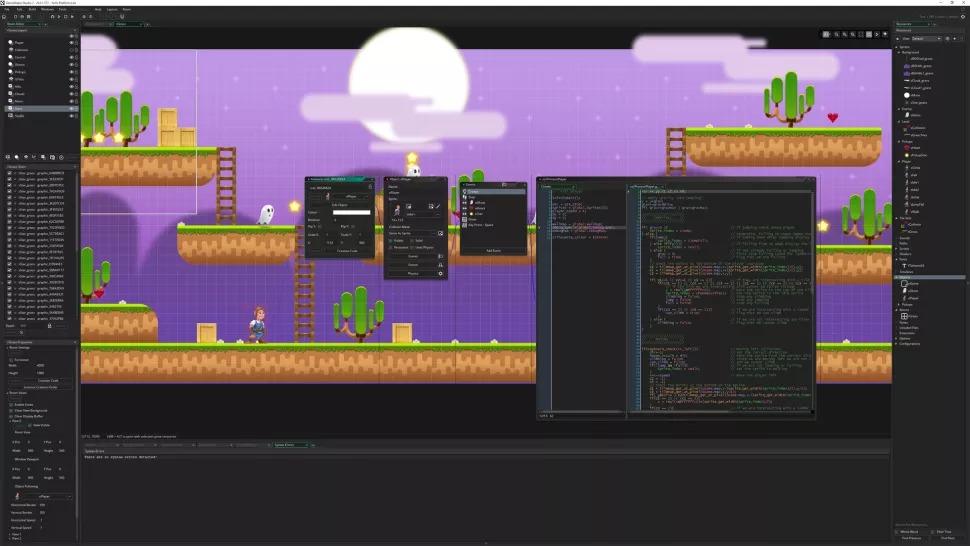
\includegraphics[height = 210pt]{2d_game_dev.png}\end{center}
		\caption{Développement de jeux 2D}
		\label{Développement de jeux 2D}
	\end{figure}
	Si vous êtes des passionnés de jeux dans le plan (2D) vous aurez besoin d'au moins un processeur avec 
	des graphiques intégrés DX11. Il s'agit de processeurs Core de 3ème génération avec Intel HD Graphics
	4000/2500 ou bien un processeur dual-core 64 bits et 2 Go de RAM. Examinons les composants, en passant 
	par les facettes importantes de chacun.
	\begin{figure}[h]
		\begin{center}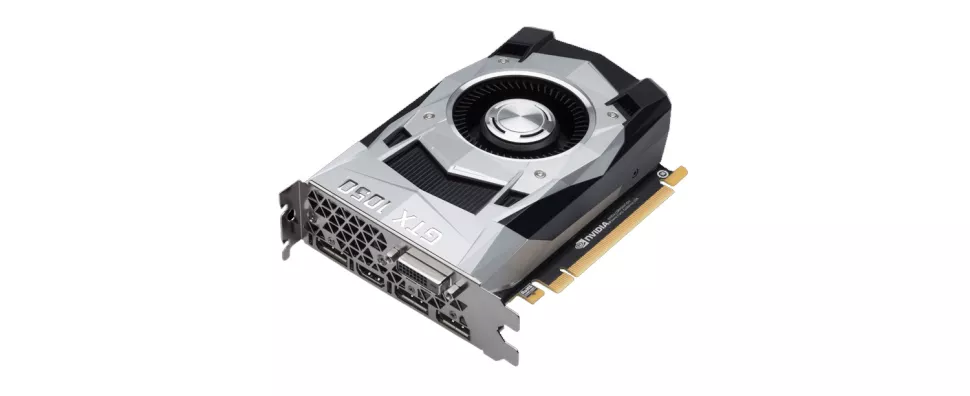
\includegraphics[height = 125pt]{2d_graphic_card.png}\end{center}
		\caption{Nvidia GeForce GTX 1050 Ti}
		\label{Nvidia GeForce GTX 1050 Ti}
	\end{figure}
	\newpage \begin{itemize}
		\item[• La carte dédiée est une priorité;]
		\item[• Compatible DirectX 11 et versions ultérieures;]
		\item[• Au moins 2 Go de RAM vidéo.]
	\end{itemize}
	Le matériel graphique est autant une priorité dans le développement que dans le jeu, voire plus si vous
	travaillez avec de puissants moteurs 3D ou en VR. Mais pour des projets simples en 2D, vous pouvez vous
	en sortir en utilisant les graphiques intégrés de votre CPU s'ils répondent aux spécifications minimales
	du moteur. Une carte dédiée est donc un luxe plutôt qu'une exigence, mais un luxe hautement recommandé. 
	En général, plus vous disposez de puissance de traitement graphique et de mémoire, plus votre expérience
	dans un environnement de développement sera fluide. Comme pour les jeux, il est toujours logique
	d'investir dans la dernière génération de matériel disponible, nous avons donc choisi une GTX 1050 Ti
	bas de gamme avec 4 Go de mémoire GDDR5 et compatibilité DX12, pour 160\$.
	\begin{figure}[h]
		\begin{center}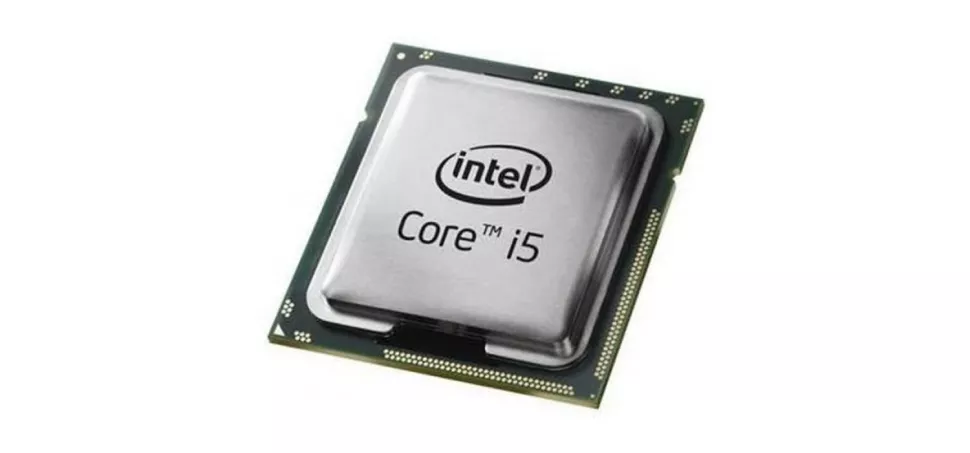
\includegraphics[height = 150pt]{2d_cpu.png}\end{center}
		\caption{Intel Core i5 7400}
		\label{Intel Core i5 7400}
	\end{figure}
	\begin{itemize}
		\item[• Un processeur plus rapide accélère les temps de compilation/rendu;]
		\item[• Au moins un Core i5;]
		\item[• Utilisez des graphiques intégrés pour les tests bas de gamme.]
	\end{itemize}
	Il y a au moins un élément de CPU-picking sur lequel il y a consensus: optez pour au moins un Core i5. À
	ce stade, vous disposez à la fois d'une puissance de traitement décente et d'une option graphique
	intégrée raisonnablement puissante pour les tests bas gamme. Choissez de préférence, un Core i5 7400.
	L'architecture de génération actuelle est abordable avec quatre cœurs à 3 GHz et une option intégrée HD
	Graphics 630 compatible DX12.
	\begin{figure}[h]
		\begin{center}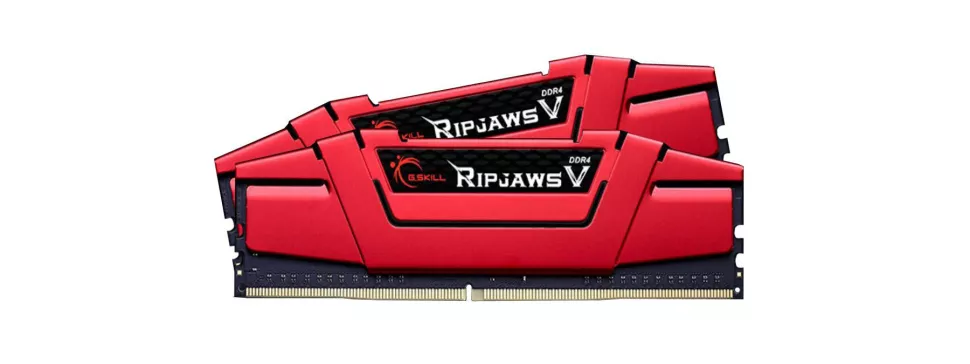
\includegraphics[height = 145pt]{2d_memory_ram.png}\end{center}
		\caption{G.Skill Ripjaws V Series 8GB}
		\label{G.Skill Ripjaws V Series 8GB}
	\end{figure}
	\begin{itemize}
		\item[• 8 Go sont suffisants pour travailler et jouer;]
		\item[• Assez de RAM est important pour le multitâche;]
		\item[• Ne vous inquiétez pas des timings RAM.]
	\end{itemize}
	Nous avons opté ici pour un ensemble de 8 Go rapide et bon marché de G.Skill, mais vous pouvez doubler
	la capacité à 16 Go pour seulement environ 50\$ de plus si vous voulez jouer en toute sécurité.
	% 3D Game developement.
	\newpage \subsubsection{\textcolor{darkgreen}{Développement de jeux 3D}}
	\begin{figure}[h]
		\begin{center}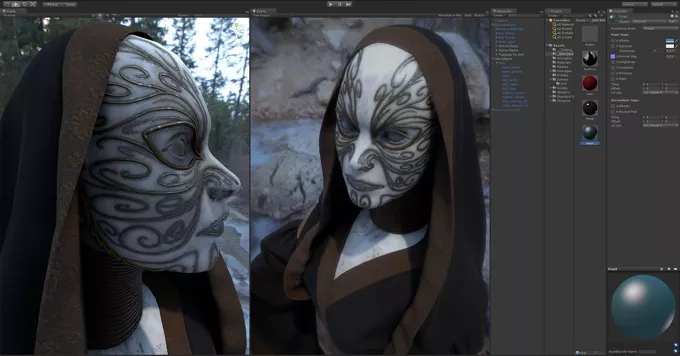
\includegraphics[height = 195pt]{3d_game_dev.png}\end{center}
		\caption{Développement de jeux 3D}
		\label{Développement de jeux 3D}
	\end{figure}
	Si vous êtes des passionnés de jeux en image de synthèse (3D) vous aurez besoin d'un processeur
	quadricœur 2,5 GHz, 8 Go de RAM et GeForce 470 GTX/Radeon 6870 HD ou supérieur est recommandé.
	\begin{figure}[h]
		\begin{center}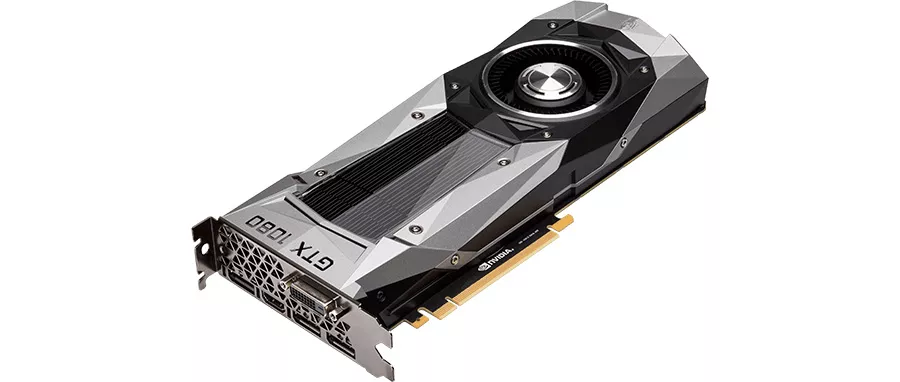
\includegraphics[height = 160pt]{3d_graphic_card.png}\end{center}
		\caption{Nvidia GeForce GTX 1080}
		\label{Nvidia GeForce GTX 1080}
	\end{figure}
	\begin{itemize}
		\item[• Carte dédiée fortement suggérée;]
		\item[• Compatible DirectX 11 et versions ultérieures;]
		\item[• Au moins 2 Go de RAM vidéo.]
	\end{itemize}
	Contrairement au développement 2D, se débrouiller avec des graphiques intégrés n'est pas aussi facile
	ici. Une carte graphique dédiée vous aidera beaucoup, en particulier dans un moteur puissant. Une très
	grande GTX 1080 sera d'une grande aide pour traiter tous les effets de post-traitement, l'éclairage et
	les ombres. Pourquoi Nvidia ? Ce n'est pas que les cartes de l'équipe verte soient nécessairement
	meilleures pour se développer. Cependant, sa position dominante sur le marché signifie que si vous
	testez votre jeu sur une carte Nvidia, vous testez sur du matériel que votre public est plus susceptible
	d'utiliser.
	\begin{figure}[h]
		\begin{center}
\includegraphics[height = 115pt]{3d_cpu.png}\end{center}
		\caption{Intel Core i7 7700K}
		\label{Intel Core i7 7700K}
	\end{figure}
	\begin{itemize}
		\item[• Un processeur rapide pour accélérer les temps de compilation/rendu lourds;]
		\item[• Au moins un Core i5 pour travailler en 3D;]
		\item[• Utilisez des graphiques intégrés pour les tests bas de gamme.]
	\end{itemize}
	Pour travailler sur des projets 3D plus exigeants, il faut passer à un Core i7 pour aider à réduire les
	temps de compilation et de rendu. Bien que plusieurs cœurs et des performances de multithreading plus
	élevées ne soient toujours pas si importants pour jouer à des jeux, les tâches créatives lourdes (et les
	logiciels vidéo comme Adobe Premium, un outil important si vous créez des vidéos de votre propre jeu)
	peuvent tirer parti de la puissance supplémentaire d'un i7.
	\newpage \begin{figure}[h]
		\begin{center}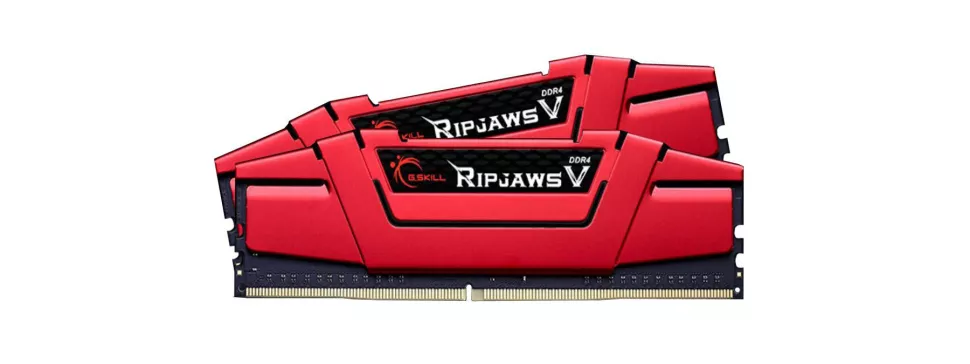
\includegraphics[height = 145pt]{2d_memory_ram.png}\end{center}
		\caption{G.Skill Ripjaws V Series DDR4-2400}
		\label{G.Skill Ripjaws V Series DDR4-2400}
	\end{figure}
	\begin{itemize}
		\item[• 16 Go prendront en charge plusieurs charges de travail lourdes;]
		\item[• Assez de RAM est important pour le multitâche;]
		\item[• Ne vous inquiétez pas des timings RAM.]
	\end{itemize}
	16 Go vous donnera la surcharge nécessaire pour en exécuter plusieurs programmes à la fois sans
	compromis. Si vous effectuez beaucoup de travaux de modélisation 3D et exécutez un moteur puissant
	simultanément, optez pour 16 Go. Si vous avez vraiment besoin d'économiser de l'argent, vous pouvez
	passer à 8 Go pour environ 50\$ de moins.
	% Other components.
	\subsubsection{\textcolor{darkgreen}{Autres composants}}
	\begin{itemize}
		\item[• Obtenez un SSD. Sérieusement;]
		\item[• Les grands écrans facilitent le flux de travail;]
		\item[• Envisagez une configuration à deux moniteurs.]
	\end{itemize}
	Avec les composants sous le capot pris en charge, dépensez le reste de votre budget sur un beau grand
	écran. Ensuite, dépassez votre budget et achetez-en un autre. L'exécution de plusieurs programmes sur un
	petit panneau n'est pas amusant et ralentit sérieusement le flux de travail. Vous pouvez dépenser
	beaucoup ou peu pour un moniteur. L'autre composant que nous n'avons pas encore abordé est le stockage à
	semi-conducteurs. Pour certains, il peut être impensable de construire un système en utilisant
	uniquement des disques durs à l'ancienne, mais cela vaut la peine de le préciser: travailler à partir
	d'un SSD va vraiment, vraiment aider. Les projets de développement de jeux peuvent prendre beaucoup de
	place et nécessiter des dizaines de milliers d'actifs individuels. Si vous retirez ces ressources d'un
	disque dur ou devez les transférer entre les disques parce que vous manquez d'espace, il est temps de
	passer à un SSD.
	% Conclusion.
	\subsubsection{\textcolor{darkgreen}{Conclusion}}
	De tout ce qui précède, on retient que vue le travail gigantesque auquel doit faire face le développeur,
	des progiciels dite \textbf{moteur de jeu} ont été misent en place pour faciliter la vie à ces derniers
	dans leurs développements. Néanmoins, pour utiliser ces moteurs, il faut disposé des bons matériaux afin
	de donner une expérience complète lors des développements.

	% Area problems.
	\section{\textcolor{darkred}{Les problématiques du domaine}}
	% Game engine problems.
	\subsection{\textcolor{darkorange}{Le système existant}}
	Les systèmes de moteur de jeu ont fait la une des journaux il y a seulement quelques années. Avant 
	l'apparition des technologies de moteur de jeu, les systèmes existants étaient souvent développés en
	tant que systèmes de réalité augmentée virtuelle pour gérer des tâches spécifiques telles que
	\textbf{NPSNET}, \textbf{DIVE} et \textbf{SPLINE}. Ainsi, toute modification nécessitait un changement
	brutal de l'environnement de programmation et de l'architecture. À mesure que la technologie des moteurs
	de jeu mûrit et devient plus flexible, la mise en œuvre d'un environnement 3D deviendra plus facile.
	Malgré ces améliorations, les compétences en programmation restent une préoccupation et sabotent
	généralement les développeurs qui souhaitent créer des environnements complexes. Les développeurs de
	jeux ont généralement des compétences avancées en programmation et bloquent souvent le système contre
	les manipulations ou les abus par l'utilisateur, ce qui complique encore la tâche. La plupart des
	moteurs de jeu sont limités à des tâches spécifiques et leurs fonctionnalités sont généralement
	associées à des caractéristiques de jeu spécifiques. Ainsi, développer des extensions ou des
	modifications qui obligent un moteur de jeu à adopter une nouvelle classe d'applications est quasiment
	impossible. Récemment, de nombreuses techniques et approches de programmation telles que le langage de
	modélisation de réalité virtuelle \textbf{VRML}, \textbf{OpenGL}, \textbf{DirectX}, \textbf{X3D} et
	\textbf{MPEG-4} ont été développées pour créer des applications de jeux. Mais, bon nombre de ces
	nouvelles méthodes ne peuvent pas fournir de support natif pour étendre les jeux existants. De plus, la
	réalisation d'un jeu fait appel à plusieurs éléments. Cependant, au cours de son développement, tous ces
	éléments ne viennent pas forcément du moteur (les models 2D ou 3D, les textures, les effets sonores, les
	animations etc...). Toutes ces données numériques proviennent souvent d'ailleurs. Par exemple pour
	donner une couleur réelle à un ou plusieurs matériaux, le développeur est plier d'aller lui-même
	chercher cette texture sur une autre platforme. Mieux encore, le personnage principal du jeu a été
	entièrement modélisé dans un autre environnement dédié à la modélisation, afin d'être importé dans le
	moteur. Ce qui signifie qu'avoir le moteur simplement est insufisant pour faire un jeu complet. On a
	donc bésoin d'autres outils spécialisés dans chacun des secteurs du développement. Le moteur représente
	la pièce maîtresse du développement d'un jeu vidéo. De tout ce qui précède, on ne peut pas tout faire
	avec un moteur de jeu. C'est donc un point qui pénalise ce dernier.
	% Game dev problems.
	\subsection{\textcolor{darkorange}{Le développement de jeux vidéo}}
	Avec la participation croissante des jeux numériques dans l'économie et notre société, l'attention 
	portée à ce sujet dans le domaine académique s'est également accrue. Cependant, le domaine du génie
	logiciel et, plus précisément, les processus de développement de jeux semblent être oubliés par les
	chercheurs. De plus, les développeurs de jeux et les grandes entreprises de jeux préfèrent garder leurs
	processus et méthodologies pour eux-mêmes. Des études et des rapports professionnels ont montré le 
	«\textit{visage laid}» derrière l'industrie du jeu vidéo. Les temps de crise et la forte pression
	pendant le développement sont traités comme des pratiques normales dans la vie d'un développeur de jeux.
	Notez qu'au cours du dévéloppement d'un jeu, il y a certaines choses qu'on ne peut ignorées, car celles-
	ci sont indispensables pour le dévéloppement de ce dernier. On pourrait dire qu'elles représentent les
	piliers centrales de tous le dévéloppement. Dans un jeu qui se respecte, on peut constaté la présence de
	certains systèmes à savoirs:
	\begin{itemize}
		\item[+] Le système de sauvegarde et de chargement de données;
		\item[+] Le gestionnaire d'optimisation graphique à travers la méthode d'\textbf{Occlusion Culling};
		\item[+] Le gestionnaire des configurations globales;
		\item[+] Le gestionnaire des cinématiques;
		\item[+] Le gestionnaire des différentes langues;
		\item[+] etc...
	\end{itemize}
	Cependant, l'implémentation de chacun de ces systèmes demandent beaucoup du temps et de l'énergie
	surtout lorsqu'on envisage de faire quelque chose de professionnelle. Un programmeur, même professionnel 
	peut ne pas être à l’aise avec la réalisation d’un jeu vidéo. Certes, il ne sera pas démuni, mais les 
	problématiques d’un jeu vidéo sont différentes de celles rencontrées lors de la réalisation d’une 
	application «\textit{classique}». L'étude et notre expérience dans le domaine nous a montré que ces 
	systèmes sont incontournable au cours du développement. Imaginé que le développeur est parvenu à mettre 
	en place les différents systèmes nécessaire pour la réalisation de son application. Lorsque ce dernier 
	se penchera sur un autre projet, il sera dans l'obligation de réimplémenter chaque système un à un,
	encore et encore en fonction de la nature du jeu auquel il est en train de développé. Ce qui serais
	pénible et fastidieux sans compté que la réalisation de ces derniers peuvent s'avérer être difficile. On
	voit bien que la mise au point d'un jeu vidéo demmande énormément beaucoup d'effort à son élaborateur.
	Les différents systèmes que nous avons évoqués plus haut ne sont présent dans aucun des moteurs de jeu,
	même pas dans ceux les plus connu. Peut être que les entreprises de jeu vidéo ont déjà développé un tel
	outil. Si c'est le cas, c'est qu'ils l'on certainement rendu propriétaire et privé. Par conséquant
	inaccessible à tout le monde.	
	
	% Genus idea.
	\section{\textcolor{darkred}{Proposition de solutions}}
	En ce qui concerne les problèmes liés aux moteurs de jeux, des solutions ont été apportées à travers
	l'utilisation des systèmes comme \textbf{Bamboo} et \textbf{JADE} pour surmonter les limitations,
	induites par les moteurs de jeux et la plate-forme de développement interconnectés. De plus malgré
	l'impuissance des moteurs face à certaines choses, on arrive qu'en même à rassemblé les différents
	éléments dont-on a bésoin pour développer l'application grâce à des services et des progiciels comme:
	\textit{Blender}, \textit{Adobe Fuse CC}, \textit{Maya}, \textit{Cinema 4D}, \textit{Sweet Home 3D},
	etc...\\
	Par contre, on ne peut pas en dire autant au niveau des difficultés rencontrées au cours de
	l'élaboration des jeux vidéo. Plus précisement dans le domaine des scriptages et des programmations.
	Réalisé un jeu vidéo n'est pas une tâche facile, surtout si celui-ci doit être fait dans les règles de
	l'art. La nécessité d'implémenter les piliers de bases à chaque projet de développement, nous amène à 
	mettre en place des mesures pour régler ce problème. C'est dans ce optique que nous avons décidé de
	réaliser un \textbf{framework} sous le nom de \textbf{Godot Mega Assets} vue la redondance de ces
	systèmes. Ce système s'addressera à l'industrie du jeu vidéo et plus précisement aux programmeurs
	(développeurs) du domaine.
	% System clarification.
	\subsection{\textcolor{darkorange}{Clarification du système à mettre en place}}
	% Framework definition.
	\subsubsection{\textcolor{darkgreen}{Définition d'un framework}}
	En programmation informatique, un framework (appelé aussi \textbf{infrastructure logicielle, socle
	d'applications, infrastructure de développement, ou cadre d'applications}) désigne un ensemble cohérent
	de composants logiciels structurels, qui sert à créer les fondations ainsi que les grandes lignes de
	tout ou d’une partie d'un logiciel (architecture). En programmation orientée objet, un framework est
	typiquement composé de classes mères qui seront dérivées et étendues par héritage en fonction des
	besoins spécifiques à chaque logiciel qui utilise le framework. Avec un framework orienté objets, le
	programmeur qui utilise le framework pourra personnaliser les éléments principaux du programme par
	extension, en utilisant le mécanisme d'héritage: créer des nouvelles classes qui contiennent toutes les 
	fonctionnalités que met en place le framework, et en plus ses fonctionnalités propres, créées par le 
	programmeur en fonction des besoins spécifiques à son programme. Le mécanisme d'héritage permet 
	également de transformer des fonctionnalités existant dans les classes du framework. Un framework se 
	distingue d'une simple bibliothèque logicielle principalement par:
	\begin{itemize}
		\item[•] Son caractère générique, faiblement spécialisé, contrairement à certaines bibliothèques, un 
		framework peut à ce titre être constitué de plusieurs bibliothèques, chacune spécialisée dans un 
		domaine. Un framework peut néanmoins être spécialisé, sur un langage particulier, une plateforme 
		spécifique, un domaine particulier: communication de données, data mapping, etc...;
		\item[•] Le cadre de travail qu'il impose de par sa construction même, guidant l'architecture 
		logicielle voire conduisant le développeur à respecter certains patrons de conception; les 
		bibliothèques le constituant sont alors organisées selon le même paradigme.
	\end{itemize}
	Un framework est conçu en vue d'aider les programmeurs dans leur travail. L'organisation du framework 
	vise la productivité maximale du programmeur qui va l'utiliser en vue de réduire les coûts de 
	construction et maintenance du programme. Le contenu exact du framework est dicté par le type de 
	programme et l'architecture cible pour lequel il est conçu. On trouve différents types de frameworks:
	\begin{itemize}
		\item[•] Frameworks d'infrastructure système: Pour développer des systèmes d'exploitation, des 
		interfaces graphiques, des outils de communication (exemple: \textit{Framework .Net, Struts});
		\item[•] Frameworks d'intégration intergicielle (\textit{middleware}): Pour fédérer des applications 
		hétérogènes. Pour mettre à disposition différentes technologies sous la forme d'une interface unique 
		;
		\item[•] Frameworks d'entreprise: Pour développer des applications spécifiques au secteur d'activité 
		de l'entreprise;
		\item[•] Frameworks de gestion de contenu: Ce sont les fondations d'un système de gestion de contenu 
		pour la création, la collecte, le classement, le stockage et la publication de «biens numérisés».\\
	\end{itemize}
	Les frameworks sont donc conçus et utilisés pour modeler l'architecture des logiciels applicatifs, des 
	applications web, des \textit{middlewares} et des composants logiciels. Ils sont acquis par 
	les informaticiens, puis incorporés dans des logiciels applicatifs mis sur le marché. Ils sont par 
	conséquent rarement achetés et installés séparément par un utilisateur final. Les principaux avantages 
	des frameworks sont la réutilisation de leur code, la standardisation du cycle de vie du logiciel 
	(spécification, développement, maintenance, évolution). Ils permettent de formaliser une architecture 
	adaptée au contexte étudié et tirent parti de l'expérience des développements antérieurs.
	% System sources.
	\subsubsection{\textcolor{darkgreen}{Les sources du système}}
	\textbf{Godot Mega Assets} sera réalisé sur un langage de programmation: Le \textbf{\textit{GDScript}}
	lié à un moteur de jeu: \textbf{Godot}. Développé par \textbf{Okam Studio}, ce progiciel gratuit, permet
	d'exporter ses projets sur consoles (\emph{Wii}, \emph{PS3}, \emph{PS Vita}, \emph{Nintendo 3DS}), les
	mobiles (\emph{Android}, \emph{iOS}, \emph{BBX}) et les PC (\emph{Windows}, \emph{Linux} et \emph{Mac OS
	X}). L'éditeur est également disponible sur \textit{Windows}, \textit{Mac OS X} et \textit{Linux}.\\
	\begin{center}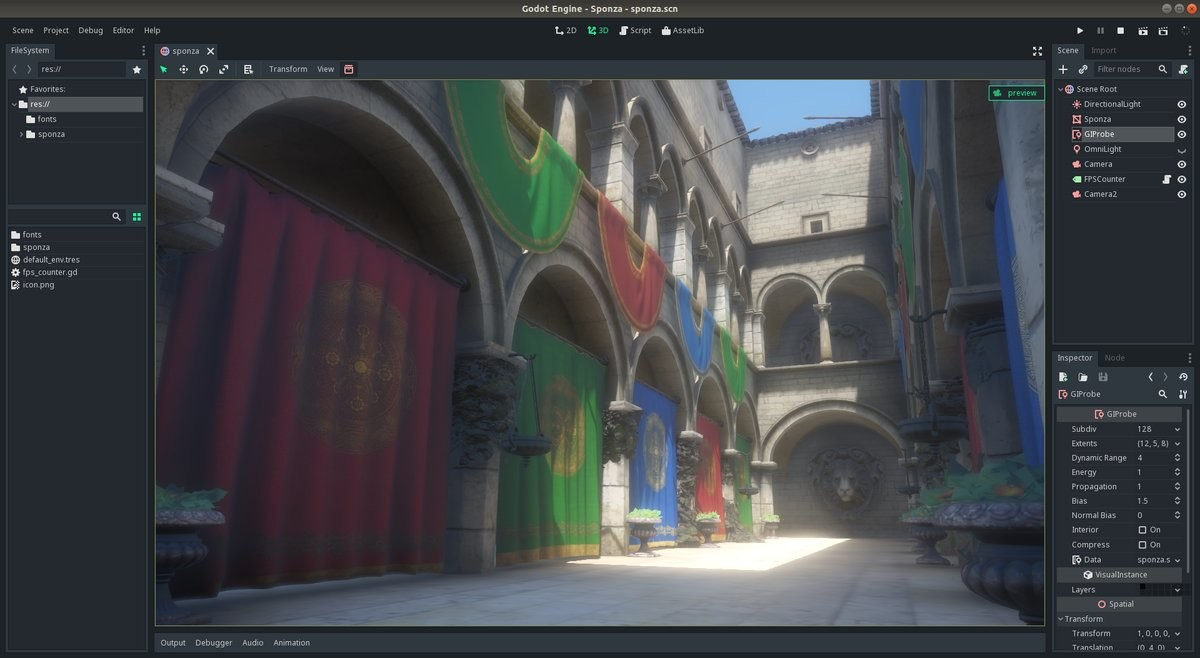
\includegraphics[width = 330pt]{godot_screenshot.jpeg}\end{center}
	Les fonctionnalités sont proches de celles que l'on peut retrouver sur le moteur \textit{Unity}, bien
	qu'il y un peu moins de choses pour la partie 3D, mais plus sur la partie 2D et le débogage. Finalement,
	le moteur propose un langage de script proche de
	\href{https://www.ionos.fr/digitalguide/sites-internet/developpement-web/tutoriel-lua/}{\textcolor{blue}
	{Lua}} et de \href{https://docs.python.org/3/}{\textcolor{blue}{Python}}. Pour plus d'informations, vous
	pouvez consulter ce lien:\\\href{https://docs.godotengine.org/fr/stable/about/faq.html}{\textcolor{blue}
	{https://docs.godotengine.org/fr/stable/about/faq.html}}\\
	\textbf{\textit{Notre système sera uniquement compatible qu'a ce moteur et ne pourra qu'être utilisé que
	dans ce moteur}}. Cette décision à été prise en se basant sur le caractère unique et complexe des
	moteurs de jeux. De plus \textbf{Godot} fait parti des moteurs de jeux modernes et les plus populaire,
	car utilisé par plusieurs développeurs partout dans le monde avec une documentation complète.
	% Future system goals.
	\subsubsection{\textcolor{darkgreen}{Les objectifs du système}}
	\textbf{Godot Mega Assets} aura pour objectif de faciliter certaines tâches aux développeurs et plus
	précisement à la mise en place des systèmes redondants au cours de la réalisation de leurs jeux vidéo.
	Cela leur permettra ainsi de se focaliser sur l'éssentiel dans leurs développements.
	% System global features.
	\subsubsection{\textcolor{darkgreen}{Les fonctionnalités globales du système}}
	\textbf{Godot Mega Assets} offrira aux développeurs:
	\begin{itemize}
		\item[+] Une structure universelle de développement facile et rapide à appréhendé;
		\item[+] La possibilité d'étendre les fonctionnalités initialement proposées par le système;
		\item[+] Des modules, tous spécialisés dans une catégory donnée en fonction du problème à resoudre;
		\item[+] Une documentation complète sur le fonctionnement du système ainsi que ces modules;
		\item[+] La compatibilité des projets réalisés avec le système sur toutes les plate-formes cible;
		\item[+] Une architecture réalisée sur la base des jeux vidéo professionnels.
	\end{itemize}
	% System reactions.
	\subsubsection{\textcolor{darkgreen}{Les interactions liées au système}}
	Les différentes interactions qui seront éffectuées sur le framework seront:
	\begin{itemize}
		\item[•] Importer le module dont-on veut utilisé (via du code ou grâce au moteur de jeu);
		\item[•] Modifier ou récupérer la ou les valeur(s) des propriétés associées à un module (en codant);
		\item[•] Appeler des méthodes renvoyant soit quelque chose, soit rien (en codant);
		\item[•] Ecouter le(s) événement(s) associé(s) à un module donné (en codant);
		\item[•] Utiliser les fonctionnalités offertes par les noyaux du framework. Par exemple, créé son
		propre module ou faire des appelles statiques.
	\end{itemize}
	Toutes ces actions seront faites par le développeur lui-même en fonction de ses bésoins.
	\textbf{\textit{L'utilisateur de ce produit doit être un programmeur ayant un niveau intermédiaire en
	programmation et également avoir une petite expérience en développement de jeux vidéo.}}
	% Framework requirements.
	\subsection{\textcolor{darkorange}{Les ressources néccessaires à l'établissement du système}}
	Avant d'éffectuer un travail, il faut s'assurer que l'on dispose des équipements nécessaires à sa
	réalisation. L'établissement de notre système fera appel aux ressources suivantes:\\
	\textbf{Les ressources matérielles} (\textit{Hardware}):
	\begin{itemize}
		\item[>>] Trois manettes joystick dont le premier respecte les conventions de la \emph{PlayStation},
		la seconde, celles de la \textit{Xbox} et la troisième, celles de la \textit{Nintendo Switch};
		\item[>>] Un clavier et une souris;
		\item[>>] Un dispositif permettant l'accès à une connexion internet (modem, wifi, etc...);
		\item[>>] Une mémoire \textit{RAM} d'une capacité de 8GB;
		\item[>>] Une carte graphique \textit{NVIDIA GeForce 8200M G};
		\item[>>] Un \textit{CPU} de type \textit{Intel Core 2 Duo E8400};
		\item[>>] Un moniteur ou écran PC;
		\item[>>] Un deuxième ordinateur présentant les mêmes caractéristiques que celles citées
		précédemment.
	\end{itemize}
	\textbf{Les ressources logicielles} (\textit{Software}):
	\begin{itemize}
		\item[>>] Un système d'exploitation (Windows ou Linux);
		\item[>>] Un logiciel de traitement d'image. Nous suggérons le logiciel \textit{Inkscape};
		\item[>>] Un logiciel de modélisation graphique. Ici nous avons choisi \textit{UMLet} qui un est
		logicielle libre et open source d'outils \textbf{UML} avec une simple interface utilisateur.
		On peut contruire facilement et rapidement des diagrammes \textbf{UML} et les exportés au format
		\textit{.eps, .pdf, .jpg, .svg}, etc..., Envoyer ensuite ces diagrammes en utilisant
  		\textit{Eclipse} et créé de nouveaux éléments \textbf{UML} personnalisés. \textit{UMLet} est
  		disponible sur \emph{Windows}, \emph{OS X} et \emph{Linux}. Il sera donc notre logicielle de
  		représentation graphique;
  		\item[>>] Un moteur de jeu. Nous recommandons fortement \textbf{Godot};
  		\item[>>] Un navigateur web. De préférence \textit{Chrome} ou \textit{Firefox};
  		\item[>>] \emph{DirectX 11} ou \emph{DirectX 12} uniquement si le système d'exploitation utilisé est
  		\textit{Windows};
  		\item[>>] Un éditeur de code comme \textit{VScode}, \textit{Sublim}, \textit{Atom}, etc...;
  		\item[>>] Un framework \textit{Backend} comme \textit{Django}, \textit{Flask}, \textit{Nodejs},
  		etc...;
  		\item[>>] Un hébergeur web comme \textit{Heroku}, \textit{GitHub}, \textit{GitLab}, etc...;
  		\item[>>] Un service de traduction comme \textit{Google}, \textit{Yandex}, \textit{Deepl}, etc...
	\end{itemize}
	\textbf{Les ressources personnels} (\textit{Main d'oeuvre}):
	\begin{itemize}
		\item[>>] Des développeurs du domaine des jeux vidéo;
		\item[>>] Des spécialistes sur les traitements sonores;
		\item[>>] Des spécialistes de l'intéligence artificiel;
		\item[>>] Des développeurs spécialisés dans la réalisation de \textbf{\textit{Shader}};
		\item[>>] Des développeurs web (\textit{Frontend} et \textit{Backend}) ou \textit{Fullstack};
		\item[>>] Des mathématiciens et physiciens;
		\item[>>] Des traducteurs;
		\item[>>] Des spécialistes compilateur.
	\end{itemize}
	% Money evaluation.
	\subsection{\textcolor{darkorange}{Les avantages de l'utilisation du système}}
	En utilisant \textbf{Godot Mega Assets}, vous bénéficerez des avantages suivants:
	\begin{itemize}
		\item[-] La réduction des coûts de maintenance grâce à la structure générique offerte par le
		framework;
		\item[-] Une optimisation des heures de travail grâce au caractère générique des modules du
		framework;
		\item[-] La capacité de développer des jeux simples, intermédiaires, avancés, complexes et
		professionnels;
		\item[-] Un système souple, optimisé et adapté à diverses plate-formes;
		\item[-] La réduction des coûts de développements et une maximisation des bénéfices grâce au moteur
		gratuit utilisé par le framework;
		\item[-] La réduction de la main d'oeuvre grâce à la qualité des services fournient par le
		framework.
	\end{itemize}
	\textbf{\textit{Le framework est open source et conçut pour être librement utilisé.}}
	% Framework spécifications.
	\subsection{\textcolor{darkorange}{Les exigences du système}}
	La réalisation de \textbf{Godot Mega Assets} doit respecter les exigences suivantes:\\
	\textbf{Les modules centraux} (\textit{noyaux}):
	\begin{itemize}
		\item[+] \textcolor{darkgreen}{MegaAssets};
		\item[+] \textcolor{darkgreen}{Module};
		\item[+] \textcolor{darkgreen}{Destructible};
		\item[+] \textcolor{darkgreen}{Indestructible};
		\item[+] \textcolor{darkgreen}{Saveable};
		\item[+] \textcolor{darkgreen}{Recordable}.
	\end{itemize}
	\textbf{Les modules de l'intéligence artificiel} (\textit{IA}):
	\begin{itemize}
		\item[+] \textcolor{darkgreen}{AIActionSimulatorFx};
		\item[+] \textcolor{darkgreen}{AIMotionVectorFx}.
	\end{itemize}
	\textbf{Les modules utilisant la caméra}:
	\begin{itemize}
		\item[+] \textcolor{darkgreen}{CameraControlFx};
		\item[+] \textcolor{darkgreen}{CameraEffectsFx};
		\item[+] \textcolor{darkgreen}{CutSceneFx};
		\item[+] \textcolor{darkgreen}{OcclusionCullingFx}.
	\end{itemize}
	\textbf{Les modules généraux}:
	\begin{itemize}
		\item[+] \textcolor{darkgreen}{AnimatorFx};
		\item[+] \textcolor{darkgreen}{ClonesBreakerFx};
		\item[+] \textcolor{darkgreen}{ControllerSensorFx};
		\item[+] \textcolor{darkgreen}{CursorFx};
		\item[+] \textcolor{darkgreen}{InputControllerFx};
		\item[+] \textcolor{darkgreen}{InputGeneratorFx};
		\item[+] \textcolor{darkgreen}{LanguagesFx};
		\item[+] \textcolor{darkgreen}{PermutatorFx};
		\item[+] \textcolor{darkgreen}{SaveLoadFx};
		\item[+] \textcolor{darkgreen}{ScenesFx};
		\item[+] \textcolor{darkgreen}{SettingsFx};
		\item[+] \textcolor{darkgreen}{StandardEffectsFx};
		\item[+] \textcolor{darkgreen}{VideoRecorderFx}.
	\end{itemize}
	\textbf{Les modules de l'interface utilisateur}:
	\begin{itemize}
		\item[+] \textcolor{darkgreen}{DialogSystemFx};
		\item[+] \textcolor{darkgreen}{InventoryFx};
		\item[+] \textcolor{darkgreen}{MenuFx}.
	\end{itemize}
	\textbf{Les modules naturel}:
	\begin{itemize}
		\item[+] \textcolor{darkgreen}{FireSimulatorFx};
		\item[+] \textcolor{darkgreen}{ObjectAppearanceFx};
		\item[+] \textcolor{darkgreen}{RainSimulatorFx};
		\item[+] \textcolor{darkgreen}{TemporalCycleFx};
		\item[+] \textcolor{darkgreen}{TimeFx};
		\item[+] \textcolor{darkgreen}{WaterSimulatorFx};
		\item[+] \textcolor{darkgreen}{WindSimulatorFx}.
	\end{itemize}
	\textbf{Les modules de la physique virtuelle}:
	\begin{itemize}
		\item[+] \textcolor{darkgreen}{DestroyerFx};
		\item[+] \textcolor{darkgreen}{FrictionFx};
		\item[+] \textcolor{darkgreen}{ImpactFx};
		\item[+] \textcolor{darkgreen}{MagneticFieldFx};
		\item[+] \textcolor{darkgreen}{MotionTrailFx};
		\item[+] \textcolor{darkgreen}{MotionVectorFx};
		\item[+] \textcolor{darkgreen}{ObjectGravityFx};
		\item[+] \textcolor{darkgreen}{ObjectStateFx};
		\item[+] \textcolor{darkgreen}{ObjectWavesFx};
		\item[+] \textcolor{darkgreen}{PrefabsInstanceFx};
		\item[+] \textcolor{darkgreen}{SlicerFx};
		\item[+] \textcolor{darkgreen}{WeightQuantifierFx}.
	\end{itemize}
	\textbf{Les modules joueur}:
	\begin{itemize}
		\item[+] \textcolor{darkgreen}{AnimationControllerFx};
		\item[+] \textcolor{darkgreen}{InverseKinematicFx};
		\item[+] \textcolor{darkgreen}{MultiplayerFx}.
	\end{itemize}
	\textbf{Les modules sonores}:
	\begin{itemize}
		\item[+] \textcolor{darkgreen}{AudioControllerFx};
		\item[+] \textcolor{darkgreen}{AudioGeneratorFx};
		\item[+] \textcolor{darkgreen}{AudioRecorderFx};
		\item[+] \textcolor{darkgreen}{AudioSamplerFx};
		\item[+] \textcolor{darkgreen}{AudioSpectrumFx};
		\item[+] \textcolor{darkgreen}{AudioTrackFx}.
	\end{itemize}
\end{document}